In this modern world, photopollution data is provided by satellites so as a consequence the idea for this project came to Conor when he was pondering whether it would be possible to determine the severity of photopollution without the need of satellites. Conor was also naturally attracted to Physics and Astronomy as he had a strong proficiency and interest in both. He also lives in Blackwater. Blackwater, is a dark site and is found in the Kerry International Dark-Sky Reserve. The Kerry International Dark-Sky Reserve was designated as Ireland’s first International Dark Sky Reserve by the International Dark Sky Association.\cite{kds}
An IDA International Dark Sky Reserve is land possessing an exceptional quality of starry nights and nocturnal environment.\cite{ida}
This allowed him to pursue his interest in Astronomy without having to travel great distances to a dark site.

Hannah was interested in this project due to her passion for the environment. The relevancy of photopollution and its adverse effects on wildlife sparked her interest and she wanted to find out more about how bad it was in Munster. She also lives in a dark sky reserve and has always loved astronomy, often stargazing with her family. The photopollution calculator can be used by casual astronomers like herself.

\section{Background Research}
\subsection{Population Density and Photopollution}
Photopollution is defined as the presence of anthropogenic light in the night environment. Photopollution is different from light pollution in the sense that the former is more of a generalised term that can also deal with radio spectrum pollution meanwhile photopollution deals specifically with light pollution in the visible spectrum.\cite{photopollution}
It is important to note, however, that radio spectrum pollution also presents significant problems, chief among them being adverse effects on all radio communication services, and stargazing conditions in the radio wavelength of the electromagnetic spectrum.\cite{radiowave}

Population density is a measurement of population per unit area or unit volume.\cite{pdgeo}
For our experiment, we will use people per square kilometre (people per $km^2$) as the unit of measurement for population density.

\subsection{The Problem with Photopollution}
Photopollution from villages, towns, and cities has developed into a major problem. One hundred years ago, the majority of the world could look up and see hundreds of thousands of stars scattered across the Milky Way Galaxy. People today, however, can no longer see celestial objects such as stars and planets without having to travel great distances to reach a dark site. 60\% of Europeans and 80\% of Americans can no longer see the Milky Way Galaxy. Dan Duriscoe of the National Park Service told Vox ``If you live in Switzerland, you would have to travel more than 1,000 kilometres to reach a dark site." Scientists estimate that nearly every part of the continental United States is, in some way affected by photopollution.\cite{vox}

It’s not only the continental Europe and the United States that are affected. According to Professor Brian Espey of TCD, only 5\% of Ireland has pristine night skies free from nighttime light. He also said that over 1/2 of Ireland’s population lives under skies so bright that the Milky Way cannot be seen.\cite{irishtimes}

This presents a huge problem for astronomers and physicists who need clear views of the sky to do their research, so their instruments have to be built in increasingly remote locations. In the future, when  photopollution even creeps into isolated corners of the world, a faint glow will shroud the sky and block out some of the wonders of our universe.\cite{vox}

Another negative aspect of photopollution is its effect on wildlife. Birds in your garden will be affected by security lighting, or even worse, by 'decorative' floodlighting illuminating trees from the base. The effects of this can be seen by birds feeding and singing after dark; their natural cycles are disturbed by strong artificial lighting.\cite{prob}
This affects Irish wildlife including many endangered species. Nocturnal animals are some of the worst affected because they can no longer tell when it is night time. Photopollution also has a major impact on species of endangered sea turtles that nest on beaches. The light from surrounding areas attracts the turtles instead of the moon light therefore negatively impacting sea turtle nesting or hatchings' ability to find the ocean.\cite{turtles}

\subsection{What has changed in the last three decades?}
Since the introduction of electric light in the 19th century, the  spread of lighting has been continuous in both amount and intensity. In Ireland, light emission has nearly doubled since 1990 - exacerbated by the Celtic tiger period. %Cite 
The population density of Ireland also increased during this period. The population density of the Republic of Ireland in 1990 was approximately 50 people per $km^2$, and in 2016, it was 70 people per $km^2$.\cite{1991}\cite{2016CensusTowns} That is an 40\% increase in population density since the year 1990. This tells us that as the population density in Ireland increased, the photopollution increased accordingly.

For context, the population density in Munster has increased from 41.98 people per $km^2$ in 1991 to 53.23 people per $km^2$ in 2016. This is a 26.79\% increase in population density since 1991.\cite{munster}

Photopollution is measured with satellites presently due to their superior accuracy over models. This is due to the fact, there are a few problems facing current models, chief among them being, the inability to define city populations which realistically model and predict light pollution remains the greatest source of uncertainty.\cite{uncertain} The first nighttime light survey in Ireland was carried out only as recently as 2015, therefore, we currently lack the data to determine whether current models used to predict photopollution would apply in Ireland. There is, however, an ongoing effort by TCD, UCD, NUIM and the Mayo Dark Skies group to do this. 

\subsection{Walker's Law and the Newling Model}
Present light pollution models are currently based on a law known as Walker's Law. Walker's Law links a city’s population with the amount of sky glow received at some distance outside of the city. The law is represented in the equation \ref{Walker}.\cite{walkerlaw} 

\begin{equation}
\label{Walker}
 I \propto PD^{-2.5}
\end{equation}

In this equation, I is the zenith sky brightness at a distance D from a city of population P. In this law, however, there may be an underlining lurking variable: population density. A model describing the urban distribution of population within cities has long been established by Newling's model. Newling's model combined previous work completed by Clark (1951) %Not Simon Clark, the YouTuber unfortunately, or his amazing thesis titled 'Quasi-Geostrophic Influence of the Polar Stratosphere on the Troposphere'.
and Tanner (1961). The equation describing the Newling model is represented in the equation \ref{Newling} 

\begin{equation}
\label{Newling}
 d_x = d_0e^{bx-cx^{2}}
\end{equation}

In this equation, $d_x$ is the population density, $d_0$ is the density at the centre, $e$ is the base of the natural logarithms, $b$ is a natural logarithm measuring the rate of change of density with distance, $c$ is the measure of rate of change, and $x$ is the distance from the city centre. The model states that population density is a quadratic exponential function of distance from the centre of the city, with the squared term in the exponent carrying a negative sign. \cite{newlingmodel}

In other words, this model tells us that in developed countries, such as Ireland and the United States, the  population density is more evenly or linearly spread out, while in cities of developing countries, population density is high in the city centre and decreases rather quickly with increased distance from the city centre. This tells us that the more developed a country/city are, the more evenly spread out" its population is. This is known as the flattening effect. Clark and Newling account for this flattening effect to the improvement in urban transportation systems.\cite{newlingmodel}

Bringing this back to photopollution then, the Newling model account of the distribution of population in cities can even be seen in photopollution maps. For example, in figure \ref{Dublin} (Dublin City, Ireland)\cite{DublinVIIRS}, there is a smooth falloff in photopollution with increased distance from the city centre, while in figure \ref {Madurai} (Madurai City, India)\cite{MaduraiVIIRS}, there is a rather sharp falloff in photopollution after a certain point. Both cities mentioned have a similar population (around 1.1 million). This matches up with what we expected in the Newling model. The population density is more evenly, or linearly distributed in the city of Dublin, while in the city of Madurai, this is not the case. 

\begin{figure}[H]
    \centering
    \caption{Nighttime Imagery of Cities as provided by the VIIRS 2018 (March) Radiance. VIIRS is one of five key instruments associated with the Suomi NPP satellite that was launched on October 28, 2011.}
    \label{fig:1}
    \begin{subfigure}{.48\textwidth}
        \centering
        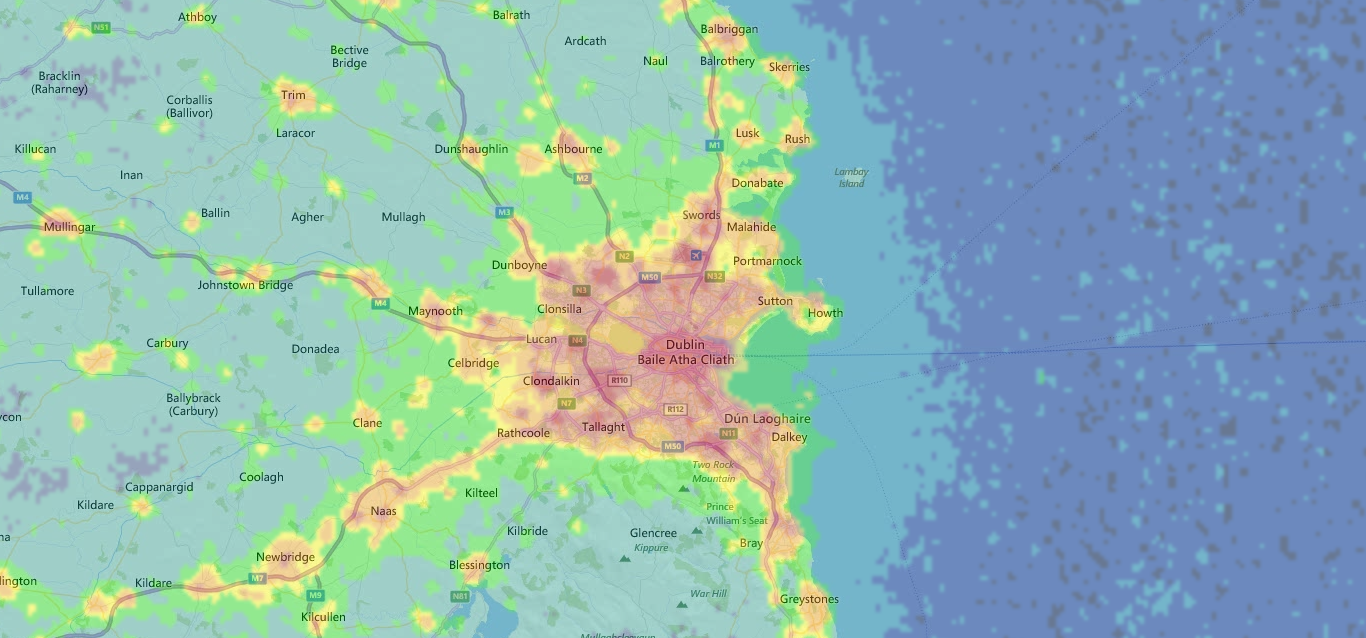
\includegraphics[width=\textwidth]{dublin}
        \caption{Nighttime Imagery of Dublin provided by the VIIRS 2018 (March) Radiance}
        \label{Dublin}
    \end{subfigure}
    \hfill
    \begin{subfigure}{.48\textwidth}
        \centering
        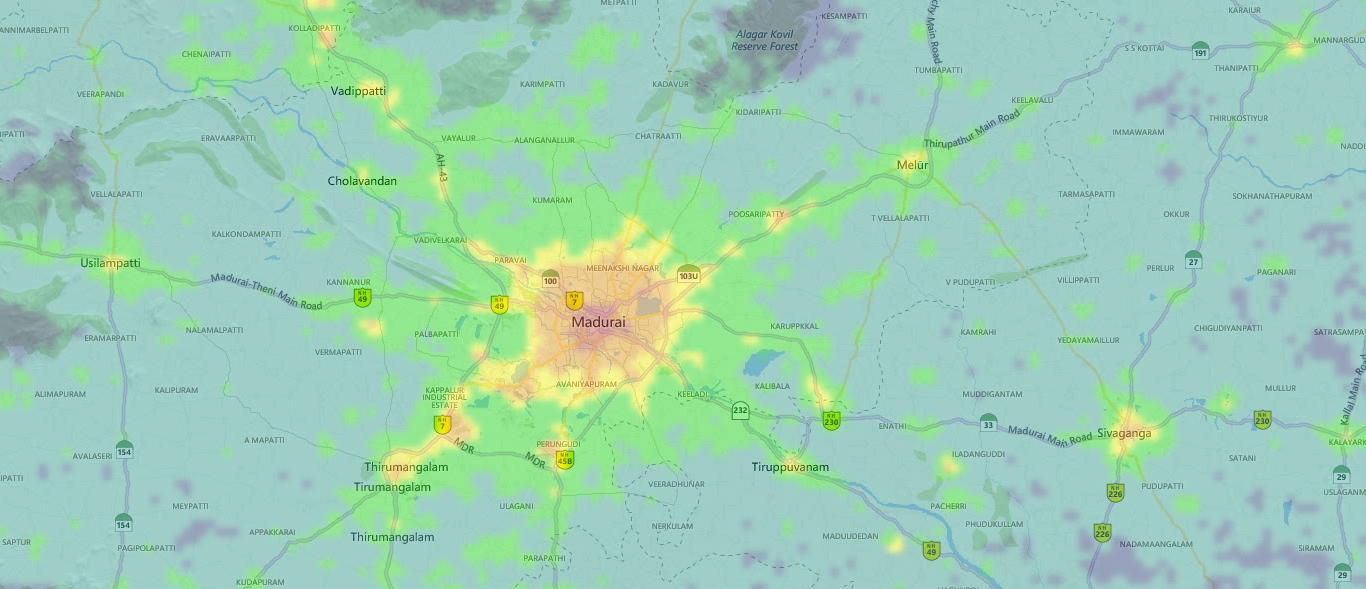
\includegraphics[width=\textwidth]{madurai}
        \caption{Nighttime Imagery of Madurai provided by the VIIRS 2018 (March) Radiance}
        \label{Madurai}
    \end{subfigure}
\end{figure}

However, Walker's Law predicts similar photopollution values in both scenarios. This is not the case, as is evident in figure \ref{fig:1}. Therefore, we can deductively conclude that the population density of an area is somehow related to the photopollution produced from that same area, and could be a better predictor of photopollution. 


\section{Hypothesis}
Our hypothesis says that a mathematical model can be created to predict photopollution in Munster based solely on population density. It assumes that population density is the main driving factor of photopollution and that all other factors are negligible. The independent variable in our case is population density and photopollution is the dependent variable.

\section{Experimental Method}
The experimental method being used to measure photopollution involves measuring the dark portion of the sky with a telescope and a photometer. Typically such measurements are made at the zenith: the point at which the sky or celestial sphere is directly above the observer.\cite{calculatelux}\cite{zenith} 
For our experiment, however, we will use a photometer app. We will use an app instead of a physical photometer as the photometer we bought proved to be incompatible with measuring through a telescope.

Measurements will be made at 20 sites located throughout Munster. These sites we plan on including are: Blackwater (Dark Site) (Kerry), Tipperary town (Tipperary), Cahir (Tipperary), Clonmel (Tipperary), Ballymacarbry (Waterford), Lismore (Waterford), Tallow (Waterford), Watergrasshill (Cork), Cork City (Cork), Macroom (Cork), Tarbert (Kerry), Kilrush (Clare), Ennis (Clare), Shannon (Clare), Limerick City (Limerick), Adare (Limerick), Newcastle West (Limerick), Tralee (Kerry), Killarney (Kerry), and Kenmare (Kerry). Population density for the different sites is provided by the Central Statistics Office.\cite{2016CensusTowns}\cite{2016ElectoralDiv}

Once all the data is collected, a relationship or trend in the data will be sought. This will be done with the help of a Python program Conor developed. We will also gather data about what the standard deviation in photopollution values is. The correlation coefficient will be used to see if there is a strong linear correlation in the data. Correlation coefficient is a measure of the strength of the linear relationship between to two sets of data. Correlation coefficient, r,  is a number in the following range: -1 $<=$ r $<=$ 1. If r is close to 1, then there is a strong positive correlation between the two sets of data. If r is close to -1, we say there is a strong negative correlation between the two sets. If r is close to 0, then there is no correlation between the two sets.\cite{am4}
The equation for the correlation coefficient is represented in the equation \ref{r}.\cite{r}

\begin{equation}
\label{r}
r = \frac{{}\sum_{i=1}^{n} (x_i - \overline{x})(y_i - \overline{y})}{\sqrt{\sum_{i=1}^{n} (x_i - \overline{x})^2(y_i - \overline{y})^2}} 
\end{equation}

We will also calculate the standard deviation. Standard deviation measures the average deviation or spread from the mean of all values in the data set. It is a reliable measure of spread, as it takes into account of all values in the set, unlike the range and interquartile range.
The equation for the standard deviation is represented in the equation \ref{stddev}.\cite{am4}

\begin{equation}
\label{stddev}
\sigma = \sqrt{\sum \frac{(x_i - \mu)^2}{n}} 
\end{equation}

\section{Ideal Outcomes}
If we are able to establish a relationship between the two variables, we will create a grading system that will determine what any photopollution value produced in any particular area would mean in relation to the stargazing conditions. Using this information, we will develop a Python program, and an app that will incorporate our model and grading system. Both applications will be published under the name Photopollution Calculator on Github, and the Google Play Store respectively.\cite{github}\cite{play_store} We will also develop a photopollution, and population density heat map of the Republic of Ireland using QGIS in order to compare them against nighttime imagery from VIIRS 2018 (March) Radiance.\cite{QGIS_software}\cite{VIIRS_compare} On each map, ROI was divided into the various electoral divisions (Electoral Boundaries were provided by the Central Statistics Office), and following which conditional formatting was used in QGIS to shade in the map.\cite{boundaries} The photopollution map was shaded based on the grading system we developed during this project.

This mathematical model proved to be reasonably accurate and could be used by amateur astronomers as a companion to a photopollution map to paint a better picture of the photopollution in the night sky. 
